\documentclass[letterpaper,11pt]{article}

\usepackage[shortlabels]{enumitem}
\usepackage[margin=1in]{geometry}
\usepackage[most]{tcolorbox}
\usepackage{hyperref}

\begin{document}
\title{{\bf Module 3: Crafting a Question} }
\author{Name: }

\date{}
\maketitle

\section{Intro}
It is finally time! In this module, you will develop a specific research question regarding all that you have learned so far.
This is really exciting! We'll walk through it, but we'll want to make sure the question is feasibly testable, and that it has provable impact and importance.
\newline
\newline
\textbf{Examples}\\
Subfield: Neuromorphic Hardware \\
Problem: Training efficiency of tranformer models \\
Can neuromorphic hardware bring significant speedups to transformer training? How much? \\
\newline
Subfield: Biologically Inspired Computing\\
Problem: Understanding the limitations and benefits of various memory forms\\
How are transformer architectures and architecture of short and long term biological memory similar or different? To what extent is the order of inputs similar and different for the two?\\
\newline
Subfield: RL\\
Problem: Unresolved physics\\
Can RL be used to rediscover laws of physics in novel ways, or potentially propose new theories of a Grand Unifying Theory?\\
\newline
\textbf{Inspiration}
For inspiration, here are some datasets that have been discussed as resources for research projects. \\
\begin{enumerate}
    \item \href{https://openneuro.org/search}{OpenNeuro} contains data from MRIs (soft tissue and structural image of the brain), EEGs (electrical activity using surface electrodes),  MEG (large scale brain activity using magnetic resonance) and more.
    \item \href{https://portal.brain-map.org/}{Allen Institute for Brain Science} releases data on the connectivity of neurons in mouse brain, neuron cell types, and more.
    \item \href{https://huggingface.co/datasets}{Hugging Face} has many various datasets, and is primarily useful for supervised or unsupervised learning tasks, but also contains many pretrained models like a fine-tunable GPT-2 (basically, the only thing you won't find is an RL environment).
    \item \href{https://openai.com/research/requests-for-research-2}{Open AI} puts out Requests for Research, which have really nice open source tools to help get started, so taking a look at these would be a great place to start!

\end{enumerate}

\section{Brainstorming Questions}
\begin{enumerate}
    \item 
    First, you will have to brainstorm specific questions. For this -- you guessed it -- you will \textbf{meet with your team}. Please come up with at least 5 potential research questions based on the information and questions you have gathered about your subfield. You may also list questions about a subfield from a former week that you did not select if you feel passionately about them. When you are done brainstorming, rank them in order of preference with your group.
    \begin{tcolorbox}
TODO: Your answer here
\newline
\newline
\newline
\newline
\newline
\newline
\newline
\newline
\newline
\newline
\newline
\end{tcolorbox}

\subsection{Viability}
\item 
Analyze the viability of your first choice of research question. First, google your question. Has it been done? No, really, \textbf{has it been done?} Type it into ChatGPT, check out the output. Go to https://arxiv.org/search/ and look it up. Report what you find, and note down any possibly useful papers for the future. 
If you find that your idea has been tried, read the current attempts and brainstorm at least 3 ways it is flawed or could be expanded. This will take time to read papers, and you may need to assign some papers for each member to read and then meet again after.
\begin{tcolorbox}
TODO: Your answer here
\newline
\newline
\newline
\newline
\newline
\newline
\newline
\newline
\newline
\end{tcolorbox}

\item
Next, brainstorm how you will test your question with the simplest possible experiment. Create a rough outline, then make a list of the required technologies and materials to complete this. \textbf{This is an iterative process, and you may need to meet with your team several times to have enough discussion and revision.} \\
Example:\\
We found that using AI to discover new physics has been explored in this paper (https://arxiv.org/abs/1810.10525). However, they used a strategy of unsupervised learning to find laws of motion for a pendulum via observation of trajectories, whereas perhaps a reinforcement learning agent with the ability to interact with the world would have more success.\\
To test if RL can discover new physics, we will need \\
1) an environment which can produce data that we want to describe with physical laws and all associated software packages \\
2) GPU compute (potentially more than available on a laptop) \\
3) more physics knowledge (professor support, physics majors, reading sources)\\
\newline
Next, rank the viability of each of your material needs from 0-10, with 10 being Easily Achievable and 0 being Impossible. Link citations where desired to back up your rating. Normalize a resulting score across all listed needs. Discuss with your group if this direction is viable. If it is not -- try again! :)
\begin{tcolorbox}
TODO: Your answer here
\newline
\newline
\newline
\newline
\newline
\newline
\newline
\newline
\newline
\end{tcolorbox}

\subsection{Impact}
\item
Now you have confidence that you have a viable research question. That's great! Now let's take a look at the impacts.

First, write three reasons you find the question interesting. Next, write three possible results of your research. What are the possible impacts of these different results? Who specifically would also be interested in these results? \\

Why do you specifically care about these possible results?\\
\begin{tcolorbox}
TODO: Your answer here
\newline
\newline
\newline
\newline
\newline
\newline
\newline
\newline
\newline
\newline
\newline
\newline
\newline
\newline
\newline
\newline
\newline
\newline
\newline
\newline
\newline
\newline
\newline
\newline
\newline
\newline
\newline
\newline
\newline
\newline
\newline
\newline
\newline
\newline
\newline
\newline
\newline
\end{tcolorbox}
\item
If you and your group have convinced yourself that this is both reasonably viable and impactful at this point, then you are ready to proceed! For this last item, you will write an email explaining your research question to someone in the field, and ask for advice and feedback! Good news! You may already have a potential list from Worksheet 2 if you stuck with a subfield that someone last week researched. \\
More good news! We already wrote you a little \href{https://docs.google.com/document/d/1ewTzFS7NR-LoHK8gTDOEQOODPNarIO47psnZr8DvSTQ/edit?usp=sharing}{email template} to save you some time here. Feel free to use it or forsake it as you see fit. \\
You're going to want to coordinate with your group a bit to make sure you don't email the same people. \\ \\
Note that researchers often take a long time to get back to people, so PhD students may be a better bet. Feel free to email as many as you can find!  Secondly, although feedback is important, we won't count on researchers being timely, and we will proceed will your chosen direction without waiting for a response. Once they respond, you may want to revise your question and that's fine!

\end{enumerate}

\begin{figure}[h]
\caption{Cool place in Alaska (Skagway) I had the good fortune of visiting for a week once upon a time. Their entire economy revolves around giant tourist cruise ships. Tuesdays were cruise ship days. Population $<$ 2,000.}
\centering
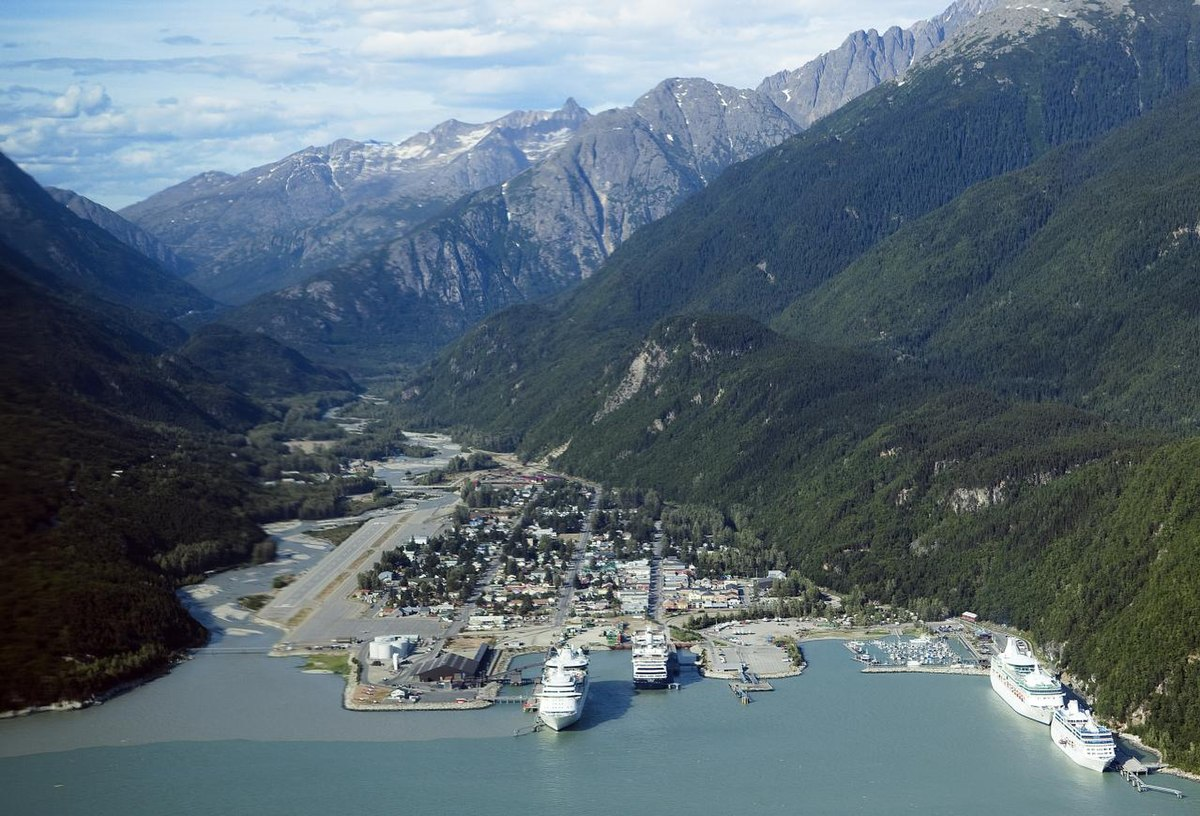
\includegraphics[width=0.5\textwidth]{skagway.jpg}
\end{figure}

\end{document}
